\documentclass[a4paper]{article}
\usepackage{amssymb}
\usepackage{graphicx}
%\usepackage{hyperref}
\usepackage{microtype}
\usepackage{amsmath, amsthm, amssymb} 
\usepackage{caption}
\usepackage{subcaption}
\usepackage{subfig}
\usepackage{xargs}
\usepackage[pdftex,dvipsnames]{xcolor}  
\usepackage[colorinlistoftodos,prependcaption,textsize=tiny]{todonotes}
\newcommandx{\mytodo}[2][1=]{\todo[linecolor=red,backgroundcolor=red!25,bordercolor=red,#1]{#2}}
\usepackage{enumitem}
\usepackage{tabu}
\usepackage{array}

\title{H09M0A P\&D Embedded Systems and Multimedia}
\author{Seppe Iven - r0370830 \\ Koen Goetschalckx - r0375967}
\begin{document} 
\maketitle
\begin{center} Yu-Hui Huang, Johan Van Rompay, Hugo Van hamme
\end{center}

\section{Introduction}
This report is about the C implementation of the MATLAB of blabla

\section{Similarities between the MATLAB and C implementation}
The C implementation of the P\&D assignment produces the exact same output as the MATLAB implementation. To achieve this, it was sometimes necessary to change the MATLAB code. For example, rounding in MATLAB was changed to behave like rounding in C. The mapping of the MATLAB and C functions is shown in table \ref{tbl:mapping}.
\mytodo{Functienamen aanpassen want dit is nodeloos verwarrend}
\begin{center}
\begin{table}
\begin{tabular}{l|r}
MATLAB & C \\
\hline
Analysis & Encode \\
Encode & Quantize \\
Decode & Dequantize \\
Synthesis & Decode \\
\end{tabular}
\caption{MATLAB to C function mapping}
\label{tbl:mapping}
\end{table}
\end{center}

\section{Differences between the MATLAB and C implementation}
\mytodo{Dees staat in execution order!}
One of the main differences between the MATLAB and C implementation is that the MATLAB implementation has access to the full .wav-file at once, while the C implementation reads the .wav-file buffer by buffer. The subband filtering and synthesis functions require previous samples to do the convolution. The quantization and dequantization functions require previous samples to calculate the moving average. To do this, both functions keep a structure that contain previous samples.

\section{Communication with an encryption group}
\mytodo{de dingen hieronder moeten in differences}
The output of the quantization function will be manipulated bit-wise \mytodo{"to compress it into as few shorts a possible"  ==> We do it in bytes (15)} and sent to an encryption group. Every sample of every subband will be quantized to 5, 4, 3 or 0 bits for the lowest to the highest subband, respectively. The quantization function however, outputs every sample as a short. The function that combines the correct bits of multiple samples into shorts, has not been written yet, but this is only seen as a formality. This is because this function is straightforward and depends on the agreement with the encryption group about the buffer size that we communicate with.

\subsection{Flexibility}
The MATLAB code offers more flexibility than the C code. In MATLAB, even the structure of the analysis and synthesis filter banks are derived from given parameters. In C however, this structure is fixed in the code.\\

Also the parameters are harder to change in the C code. In MATLAB, they are nicely combined in \texttt{generate\_some\_params.m} or \texttt{test\_some\_params.m} and given as arguments to the main routine (\texttt{run.m}). In C however, most of them are hard coded. The parameters for \texttt{quantize} and \texttt{dequantize} can be found and relatively easily changed at the the beginning of \texttt{main.c}. The parameters for the highest frequency subband can however not be changed: it is supposed that this band is completely removed. The code thus does not even quantize and dequantize this band. Changing this would require adjustments to \texttt{mainencode}, \texttt{maindecode}, \texttt{compress30samples} and \texttt{decompress30samples}. Any other change is the number of bits assigned to the subbands would require complex changes to only the latter two.\\

All the parameters for the filterbanks are as well hard to change. In MATLAB, the filters are generated based on given parameters while in C, the filters themselves must be entered. This removes the flexibility of easily changing their length or stopband attenuation. Also the amount of scaling to be done after applying the filters, is hardcoded in the C functions \texttt{encode} and \texttt{decode} and can therefore not be changed very quickly.

\subsection{Rounding and scaling}
Although the MATLAB implementation was designed to mimic C like integer operations, some false assumptions were made. Table \ref{tbl:roundingassumptions} lists these, as well as their correction and solution. The purpose of the solutions is always to make the C implementation consistent with the MATLAB implementation. The second solution might make the code a little slower, but because it is not in the critical inner loop of \texttt{convolve} (see \ref{sec:processing}) it does not make an important difference.\\

Apart from the changes mentioned in table \ref{tbl:roundingassumptions}, another change was made in MATLAB: instead of scaling the values loaded from the wav-file to let them use the full integer range, they are just multiplied with $2^15$. This is not the same when the values in the wav-file do not occupy their full available range. This change is made because in order to scale the values to the full available range, the maximum is needed. This information is not known in a real-time application, and can thus not be used.
\begin{table}[htb]
\centering
\makebox[\linewidth][c]{
\tabulinesep=1.2mm
\begin{tabu}{p{3.0cm}>{\centering\arraybackslash}p{1.7cm}p{3.5cm}>{\centering\arraybackslash}p{1.7cm}p{4cm}}
False assumption & Examples & Correction & Examples & Solution \\
\hline
\hline
MATLAB rounds integer divisions towards zero (like C) & 
	10/6 = 1 \quad (-9)/2 = -4 &
	 MATLAB rounds towards nearest integer (halves away from zero) &
	  10/6 = 2 \quad(-9)/2 = -5 &
	  MATLAB division \texttt{a/b} changed to \texttt{int16(fix( double(a)/double(b)))}.\\
\hline
C rounds the result of a division by shift towards zero &
	-9\texttt{>>}1 = -4 \quad 9\texttt{>>}1 = 4 &
	C does floor on the result&
	-9\texttt{>>}1 = -5 \quad 9\texttt{>>}1 = 4 &
	a\texttt{>>}b was replaced by \texttt{a/(1\texttt{<<}b)} in the C code.

\end{tabu}
}
\caption{False assumptions about rounding mechanisms, with their corrections and solutions}
\label{tbl:roundingassumptions}
\end{table}

\subsection{Execution order}
In MATLAB, each intermediate signal is calculated over the complete time before it is used for further calculations. This simplifies the code. It is possible because the MATLAB implementation is just for quality testing, for which the complete input signal can be known at starting time. The C code however, targets a real time-application. The complete input signal is thus not known beforehand. Waiting until the complete signal is received is impossible, because the delay would be unacceptable and the length of the input is not bounded. Therefore, the C code works buffer per buffer. It reads a specified amount of values and saves them in a buffer. On this buffer, all calculations are performed and the output is received immediately without waiting for the rest of the signal. When the output for the current buffer is calculated, a new buffer is read. The delay is thus no more than the time it takes to fill the buffer added to the intrinsic delay of the filterbank. The time needed to calculate the output of an input buffer should be negligible. 

\section{Performance enhancements}
If ipv while
Enkel encode/decode want die shit duurt lang
\subsection{Memory}
To not waste memory all these functions do work in place, meaning they can write their output on the same place as they read the input:
\begin{itemize}[noitemsep]
\item \texttt{compress30samples}
\item \texttt{combineWithoutDelay}
\item \texttt{convolve}
\item \texttt{combine}
\end{itemize}
Writing the output at the place of the input removes the necessity of reserving memory for both the input and the output. With our implementation, this comes with the cost of more complex indexing, as reading or writing 'after the end' of the array must equal reading or writing at the beginning of the array. This can easily but inefficiently be implemented by doing a modulo operation on the index. A more efficient implementation is used in the \texttt{convolve} function, as the following subsection clarifies.
\subsection{Execution time}\label{sec:processing}
After finishing a first complete and fully functioning version of the code, Visual Studio's\footnote{Microsoft Visual Studio Community 2015} CPU Sampling profiled the performance of the code. It pointed out that most time is spent in the \texttt{convolve} function. This corresponds with intuition, since it is not only the function dealing with the largest values before rescaling, but also, and more importantly, the only one with a nested loop. Table \ref{tbl:profilingresults} shows all the relevant profiling results. The numbers in these table indicate the amount of profiling samples the given function was running. These are roughly proportional to the time these functions execute. The details of \texttt{mainencode} are omitted because they are very similar to those of \texttt{maindecode}. Comparison of the unoptimized with the optimized version shows that the total amount of time is almost halved, with only improvements to \texttt{convolve} function. The mentioned \texttt{\_alldiv} function is used by the compiler for dividing long long integers.\\

\begin{table}[htpb]
\centering
\makebox[\linewidth][c]{
\begin{subtable}{0.65\textwidth}
\begin{tabular}{l|r}
Function & \#samples\\
\hline
\texttt{main} & 58818\\
\quad \quad \texttt{maindecode} & 30414\\
\quad \quad \quad \quad \texttt{decode} & 25089\\
\quad \quad \quad \quad \quad \quad \texttt{convolve} & 22835\\
\quad \quad \quad \quad \quad \quad \texttt{\_alldiv} & 1189 \\
\quad \quad \quad \quad \quad \quad others & 1062 \\
\quad \quad \quad \quad \texttt{wavpcm\_output\_write} & 3825\\
\quad \quad \quad \quad \texttt{dequantize} & 626\\
\quad \quad \quad \quad others & 874\\
\quad \quad \texttt{mainencode} & 28362\\
\quad \quad others & 42
\end{tabular}
\caption{Unoptimized}
\end{subtable}
\begin{subtable}{0.65\textwidth}
\begin{tabular}{l|r}
Function & \#samples\\
\hline
\texttt{main} & 29310\\
\quad \quad \texttt{maindecode} & 15805\\
\quad \quad \quad \quad \texttt{decode} & 10833\\
\quad \quad \quad \quad \quad \quad \texttt{convolve} & 8672\\
\quad \quad \quad \quad \quad \quad \texttt{\_alldiv} & 1225 \\
\quad \quad \quad \quad \quad \quad others & 936 \\
\quad \quad \quad \quad \texttt{wavpcm\_output\_write} & 3616\\
\quad \quad \quad \quad \texttt{dequantize} & 619\\
\quad \quad \quad \quad others & 737\\
\quad \quad \texttt{mainencode} & 13461\\
\quad \quad others & 44
\end{tabular}
\caption{Optimized}
\end{subtable}
}
\caption{Profiling results}
\label{tbl:profilingresults}
\end{table}
Figure \ref{fig:convolvefunctions} shows the unoptimized and optimized version of the \texttt{convolve} function in detail. The numbers on the left of the lines indicate the amount of samples during which each line was running. The total amount of samples spent in the inner loop is $4890 + 37999+ 979 = 43868$ for the unoptimized version and $1104+1079+199+196+1806+1009+8548+969 = 14910$ for the optimized version. The results of the optimized version also show that $1806+1009+8548 = 11363$ of the $14910$ profiling samples are spent in the last three lines. These do only essential data fetching and calculations and can thus likely not easily be more optimized. This shows that due to the optimizations, less time is spent on control and more on actual data processing.\\
\\
\begin{figure}[htpb]
\makebox[\textwidth][c]{
\begin{subfigure}[c]{.7\textwidth}
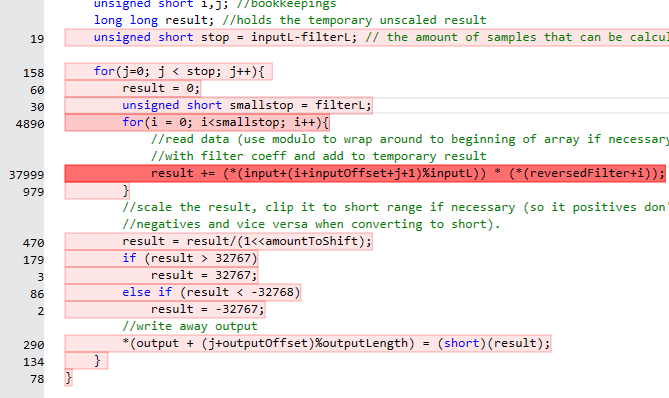
\includegraphics[width=\textwidth]{slow_convolve_cropped}
\caption{Unoptimized}
\end{subfigure}
\begin{subfigure}[c]{.7\textwidth}
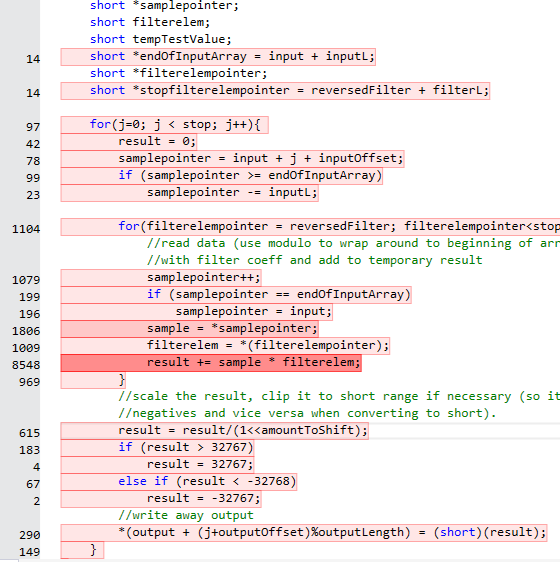
\includegraphics[width=\textwidth]{optimized_convolve_cropped}
\caption{Optimized}
\end{subfigure}
}
\caption{Details of unoptimized and optimized \texttt{convolve} functions}
\label{fig:convolvefunctions}
\end{figure}
\begin{minipage}{\textwidth}
The optimized version is derived from the unoptimized by:
\begin{itemize}
\item expanding the line of the inner loop to more substatements
\item using a pointer to the current filter element for the control of the inner \texttt{for}-loop instead of additional counter. This saves variables and replaces additions by increments.
\item keeping and incrementing a pointer to the current data sample. This saves the complex calculation of the pointer. The expensive modulo operation of that calculation is reimplemented by two simple \texttt{if}-statements.
\end{itemize}
\end{minipage}
\section{Problems while implementing the program in C}
\subsection{Pointers}\mytodo{Seppe, want mij stoort da ni echt meer, buiten dan owv laatste paragraaf in debuggin}
\subsection{Debugging}
At the start of developing the C code, development was done with basic linux tools like gedit. Debugging therefore was not more advanced than writing values to either the console or an output file and comparing them with MATLAB. These basic methods slowed down development, especially bug fixing. Therefore we switched to using advanced IDEs, like Microsoft Visual Studio or CodeBlocks. This allows using breakpoints and inspecting variables, call stacks, etc. on the fly, giving a more direct insight to what the code is doing and to where it did not correspond to MATLAB. \\

Even so, debugging was still quite a lot harder than it was with MATLAB. A first cause is the buffer per buffer operation method of the C code, compared to MATLAB calculation full signals at once. Thus, when one wants to find the cause of an error in the output, simply putting a breakpoint would also pause execution at all previous, correct, buffers. This problem was usually solved with conditional breakpoints, with conditions like checking the first value of the buffer to check if it is a buffer of interest. This made the problem manageable, but debugging was still a lot harder than in MATLAB.\\

A second cause is the way arrays are passed as arguments in our C code. This is usually done by giving both a pointer to the start of the array and the length. This however, is not recognized as an array by the used debugging tools, and thus only the first value of the array can be easily inspected by dereferencing the pointer. This problem was usually tackled finding the full array higher in the call stack. However, it remained a small annoyance.

\section{Conclusion}
This report was about the C implementation of the MATLAB of blabla

\end{document}
